\documentclass{beamer}
\usepackage[utf8]{inputenc}
\usepackage[style=authoryear, backend=biber]{biblatex}
\usepackage{listings}
\usepackage{xcolor} % Carrega o pacote para cores
\addbibresource{main.bib}

\setbeamertemplate{caption}[numbered]
\renewcommand{\figurename}{Figura}

\usetheme{Boadilla}
\usecolortheme{whale}

\title[Proposta de TCC]{Explorando algoritmos de compressão de dados: teoria, implementação e desempenho}
\author[Gustavo Kadooka]{Gustavo Yujii Silva Kadooka}
\institute[UNESP]{Universidade Estadual Paulista - Câmpus Bauru}
\date{2025}
\logo{
\includegraphics[scale=0.14]{imagens/unesp.png}}

\begin{document}
    % Slide de título
    \begin{frame}
        \titlepage  
    \end{frame}
    
    % Slide de Sumário
    \begin{frame}{Sumário}
        \tableofcontents
    \end{frame}

    %--------Introdução------
    \section{Introdução}

    % Primeiro frame
    \begin{frame}{Introdução - O que é compressão?}
        A compressão de dados é uma técnica essencial para otimizar o uso de recursos computacionais, \textbf{reduzindo
            o tamanho dos arquivos} e \textbf{acelerando a transmissão de dados}. 

        Com a crescente quantidade de dados gerados, é fundamental usar algoritmos eficientes para garantir que o armazenamento e a transferência ocorram de forma rápida e econômica.
    \end{frame}
    %------------------------

    %--------Problema--------
    \section{Problema}
    \begin{frame}{Problema} 
        Como os diferentes algoritmos clássicos de compressão de dados (Huffman, LZ77, LZW, GZIP) se comparam em termos de eficiência de compressão e tempo de execução, e qual é o impacto dessas variáveis em aplicações práticas?
        
        \begin{block}{Hipótese}
            A hipótese inicial é que os algoritmos apresentam diferenças significativas em termos de tempo de execução e
            taxa de compressão dependendo do formato de arquivo.
        \end{block}
        \begin{block}{Delimitação}
            O estudo se concentra em algoritmos de compressão sem perdas (\textit{lossless}) aplicados a arquivos de texto (\texttt{.txt}), imagens (\texttt{.bmp}) e áudio (\texttt{.wav}).
        \end{block}
    \end{frame}

    \begin{frame}{Por que \texttt{.txt}?}
        O formato de arquivo \texttt{.txt} contém apenas o texto em si, sem qualquer estrutura adicional ou informações de controle, como cabeçalhos, metadados ou formatação.

        \begin{itemize}
            \item \textbf{Sem cabeçalho}: Diferentemente de outros formatos de arquivo, como \texttt{.csv} ou \texttt{.json}, que podem incluir linhas de cabeçalho ou metadados no início do arquivo, o \texttt{.txt} não contém informações adicionais.
            \item \textbf{Armazenamento simples:} O conteúdo do arquivo \texttt{.txt} é simplesmente uma sequência de caracteres armazenados sequencialmente, o que facilita sua leitura e manipulação.
            \item \textbf{Limitações:} Não é adequado para representar dados mais estruturados, como tabelas ou documentos com informações adicionais.
        \end{itemize}
    \end{frame}

    \begin{frame}{Por que \texttt{.wav}?}
        O \texttt{.wav} (\textit{Waveform Audio File Format}) é um formato de áudio que geralmente não realiza
        compressão de dados, sendo considerado um formato de áudio sem perdas (\textit{lossless}).
        
        \begin{itemize}
            \item Armazena dados de áudio em formato bruto.
            \item Preserva a qualidade original do áudio sem nenhuma perda de informações.
            \item Frequentemente usado para gravações de alta qualidade e produção de áudio profissional.
            \item Embora o formato em si não utilize compressão, ele pode ser comprimido usando algoritmos como FLAC ou ALAC para redução de tamanho.
        \end{itemize}
    \end{frame}
    
    \begin{frame}{\textit{Header} do \texttt{.wav}}
        \begin{figure}
            \centering
            \caption{\textit{Header} do \texttt{.wav}} % Coloca a legenda acima da imagem
            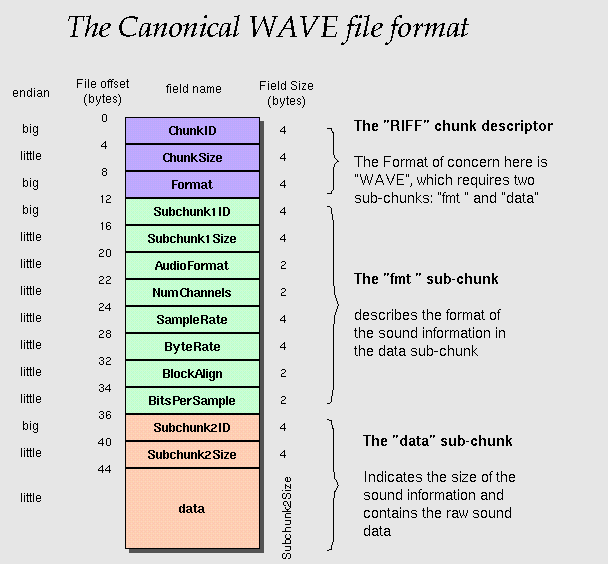
\includegraphics[width=0.55\textwidth]{imagens/wav_header.png}
        \end{figure}
        \vspace{2mm} % Espaçamento entre a imagem e a fonte
        \centering
        \textbf{Fonte:} Retirada de \textcolor{blue}{~\cite{sappwavheader}}% Coloca a fonte abaixo da imagem
    \end{frame}

    \begin{frame}{Por que \texttt{.bmp}?}
        O formato \texttt{.bmp} (\textit{Bitmap}) é um formato de imagem simples que armazena a imagem em forma de mapa de bits, geralmente sem compressão. 

        \begin{itemize}
            \item Cada pixel da imagem é armazenado individualmente, sem qualquer tipo de compressão de dados.
            \item Permite representar imagens em alta qualidade, sem perdas de detalhes ou distorções.
            \item O arquivo \texttt{.bmp} pode ser muito grande, já que não realiza compressão para reduzir o tamanho do arquivo.
            \item Embora o formato \texttt{.bmp} seja sem perdas, ele tende a ser menos eficiente em termos de tamanho de arquivo em comparação com outros formatos como \texttt{.png} (também \textit{lossless}, mas com compressão).
        \end{itemize}
    \end{frame}

    \begin{frame}{\textit{Header} do \texttt{.bmp}}
        \begin{figure}
            \centering
            \caption{\textit{Header} do \texttt{.bmp}} % Coloca a legenda acima da imagem
            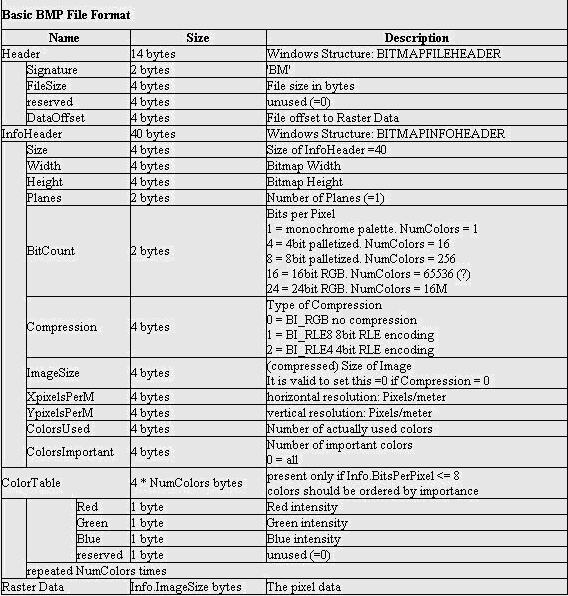
\includegraphics[width=0.45\textwidth]{imagens/bmp_header.png}
        \end{figure}
        \vspace{2mm} % Espaçamento entre a imagem e a fonte
        \centering
        \textbf{Fonte:} Retirada de \textcolor{blue}{~\cite{bmpfileformat}}% Coloca a fonte abaixo da imagem
    \end{frame}

    \begin{frame}{Entendendo Huffman}
        Técnica de compressão de dados sem perdas (\textit{lossless}) amplamente utilizada. Ele é baseado na construção de uma árvore binária, onde os símbolos com maior frequência de ocorrência são codificados com códigos mais curtos, enquanto os símbolos menos frequentes recebem códigos mais longos. 
        \begin{itemize}
            \item Contar as repetições. 
            \item Inserir ordenado numa lista. 
            \item Criar a árvore de Huffman. 
            \item Criar um dicionário.
            \item Codificar
            \item Comprimir e Descomprimir.
        \end{itemize}
    \end{frame} 

    \begin{frame}{Entendendo Huffman}
        \begin{figure}
            \centering
            \caption{Árvore de Huffman} % Coloca a legenda acima da imagem
            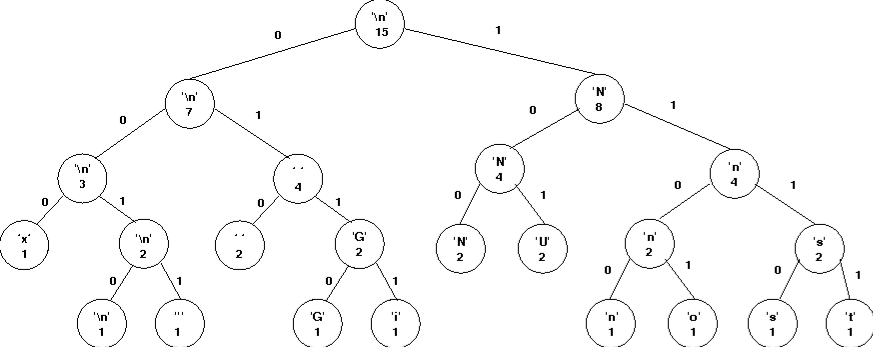
\includegraphics[width=0.9\textwidth]{imagens/huffman_tree.png}
        \end{figure}
        \vspace{2mm} % Espaçamento entre a imagem e a fonte
        \centering
        \textbf{Fonte:} Retirada de \textcolor{blue}{~\cite{islene2007lab4}}% Coloca a fonte abaixo da imagem
    \end{frame}

    \begin{frame}{Entendendo LZ77 - Lempel-Ziv 77}
        O LZ77 é um algoritmo de compressão sem perdas que utiliza um dicionário para substituir sequências repetidas de caracteres. Ele foi desenvolvido por Abraham Lempel e Jacob Ziv em 1977 e é amplamente utilizado em algoritmos de compressão como ZIP e GZIP.
        \begin{itemize}
            \item O algoritmo utiliza uma janela deslizante para identificar padrões repetidos.
            \item O dicionário contém as sequências de caracteres já vistas, e, quando uma sequência é repetida, é armazenada uma referência para a posição e o comprimento da sequência anterior.
            \item A compressão é feita substituindo sequências repetidas por um par de números: um ponteiro para a posição da sequência anterior e o comprimento da sequência.
        \end{itemize}
    \end{frame}

    \begin{frame}{Entendendo LZW - Lempel-Ziv-Welch}
        O LZW é uma variação do algoritmo LZ77, desenvolvido por Terry Welch em 1984. Ele também é um algoritmo de compressão sem perdas, mas se diferencia pela forma como gerencia o dicionário de sequências.
        \begin{itemize}
            \item Ao invés de utilizar uma janela deslizante, o LZW constrói um dicionário dinâmico durante o processo de compressão.
            \item Cada sequência de caracteres é associada a um índice no dicionário, e as sequências repetidas são substituídas pelo índice correspondente.
            \item O LZW é amplamente utilizado em formatos de compressão como GIF e TIFF.
        \end{itemize}
    \end{frame}

    \begin{frame}{Entendendo GZIP}
        O GZIP é uma ferramenta e formato de compressão de dados que combina o algoritmo LZ77 com a codificação de Huffman para compressão adicional.
        \begin{itemize}
            \item O GZIP utiliza a técnica de compressão LZ77 para remover sequências repetidas de caracteres.
            \item Em seguida, aplica a codificação de Huffman para otimizar a representação dos símbolos restantes, atribuindo códigos menores aos símbolos mais frequentes.
            \item O GZIP é amplamente utilizado para comprimir arquivos em sistemas Unix e é frequentemente usado para a compressão de arquivos de texto, como logs e arquivos HTML.
        \end{itemize}
    \end{frame}

    \begin{frame}{Por que os algoritmos clássicos?}
        Algoritmos mais recentes utilizam dos algoritmos clássicos
        \begin{itemize}
            \item \textbf{Brotli}: desenvolvido pelo Google, usado principalmente para a compressão de conteúdo da web.
            Combina técnicas, incluindo o LZ77 e o Huffman, assim como o uso de árvores de Huffman dinâmicas e modelagem estatística
            \item \textbf{Zstandard}: desenvolvido pelo Facebook para compressão em tempo real. Combina técnicas de
            compressão, incluindo o LZ77 e o Huffman.
            \item \textbf{LZMA}: LZMA é o algoritmo por trás do formato de arquivo 7z usado pelo 7-Zip. Ele é uma versão
            aprimorada do LZ77 e usa uma codificação de Huffman para compressão adicional.
        \end{itemize}
    \end{frame}

    %-------Justificativa--------
    \section{Justificativa}
    \begin{frame}{Justificativa}
    Justifica-se pela necessidade de compreender de forma aprofundada como diferentes algoritmos clássicos de compressão
    se comportam em termos de taxa de compressão e tempo de execução, analisando sua aplicabilidade em diferentes
    cenários.     

    A escolha do algoritmo de compressão adequado afeta diretamente o desempenho de sistemas de armazenamento e comunicação de dados, impactando desde a velocidade de transferência até o uso de recursos em nuvem.
        
        \begin{block}{Contribuição}
            Este estudo oferece uma análise comparativa, ajudando na escolha do algoritmo ideal para diferentes cenários de uso baseados no formato de arquivo.
        \end{block}
    \end{frame}

    %-------Objetivos--------
    \section{Objetivos}
    \begin{frame}{Objetivo Geral}
        Analisar comparativamente a eficiência dos algoritmos de compressão de dados clássicos (Huffman, LZ77, LZW, GZIP), focando na taxa de compressão e tempo de execução.
    \end{frame}
    
    \begin{frame}{Objetivos Específicos}
        \begin{itemize}
            \item Descrever os princípios teóricos dos algoritmos selecionados.
            \item Implementar os algoritmos e testar em diferentes tipos de arquivos.
            \item Fornecer recomendações para a escolha do algoritmo mais adequado.
        \end{itemize}
    \end{frame}

    \begin{frame}{Como analisar a eficiência?}
        \begin{block}{Taxa de compressão}
            \[
            T = \frac{T_{\text{original}} - T_{\text{comprimido}}}{T_{\text{original}}}
            \]
        \end{block}

        \begin{block}{Taxa de compressão média}
            \[
            T_{\text{média}} = \frac{1}{n} \sum_{i=1}^{n} \frac{T_{\text{original}, i} - T_{\text{comprimido}, i}}{T_{\text{original}, i}}
            \]
        \end{block}
    \end{frame}

    \begin{frame}{Como analisar a eficiência?}
        \begin{block}{Gráficos}
            \begin{itemize}
                \item \textbf{Barras}: 
                    \begin{itemize}
                        \item Eixo X: representa o \textbf{tipo de arquivo} (\texttt{.txt}, \texttt{.bmp},
                                \texttt{.wav})
                        \item Eixo Y: a \textbf{taxa de compressão média (\%)}.
                    \end{itemize}
                    Cada grupo de barras representa um algoritmo de compressão (Huffman, LZ77, LZW, GZIP).
                \item \textbf{Boxplots}: 
                    \begin{itemize}
                        \item Eixo X: representa o \textbf{tipo de arquivo} (\texttt{.txt}, \texttt{.bmp},
                                \texttt{.wav})
                        \item Eixo Y: a \textbf{taxa de compressão média (\%)}.
                    \end{itemize}
                \item \textbf{Dispersão} (\textit{Scatter Plot}):
                    \begin{itemize}
                        \item Eixo X: \textbf{tamanho do arquivo (KB)}.
                        \item Eixo Y: \textbf{taxa de compressão média (\%)}.
                    \end{itemize}
                \item \textbf{Linha}:
                    \begin{itemize}
                        \item Eixo X: \textbf{tamanho do arquivo (KB)}.
                        \item Eixo Y: \textbf{taxa de compressão média (\%)}.
                    \end{itemize}
            \end{itemize}
        \end{block}
    \end{frame}

    \begin{frame}{Como analisar a eficiência?}

        Com os gráficos de dispersão e de linha, podemos traçar uma \textbf{Regressão Linear} para ver se é
        aplicável.
        \[
        Y = \beta_0 + \beta_1 \cdot X + \epsilon
        \]

       \begin{block}{Coeficiente de correlação de Pearson}
           \[
                r = \frac{n \sum{xy} - \sum{x} \sum{y}}{\sqrt{[n \sum{x^2} - (\sum{x})^2] [n \sum{y^2} - (\sum{y})^2]}}
           \]
           \begin{itemize}
                \item r = 1: Correlação positiva perfeita.
                \item r = -1: Correlação negativa perfeita.
                \item r = 0: Nenhuma correlação linear.
                \item 0 < r < 1: Correlação positiva.
                \item -1 < r < 0: Correlação negativa.
           \end{itemize}
       \end{block}
    \end{frame}

    \begin{frame}{Como analisar a eficiência?}
        \begin{block}{Teste de normalidade de Shapiro-Wilk}
            \begin{itemize}
                \item Hipotese nula (\(H_0\)): Os dados seguem uma distribuição normal.
                \item Hipotese alternativa (\(H_1\)): Os dados não seguem uma distribuição normal.
            \end{itemize}
            Se o valor-p (p-value) do teste for menor que o nível de significância (geralmente 0,05), você rejeita a hipótese nula e conclui que os dados não são normais.
        \end{block}

        \begin{block}{Teste t de Student}
            \begin{itemize}
            \item O teste t de Student compara as médias de dois grupos independentes.
            \item Se o valor-p do teste t for menor que 0,05, rejeitamos a hipótese nula (não há diferença significativa entre os grupos) e concluímos que há uma diferença significativa nas taxas de compressão.
            \end{itemize}
        \end{block}
    \end{frame}

    \begin{frame}{Como será a implementação?}

        \begin{block}{\textit{Back-End}}
            A implementação do \textit{back-end} será feita utilizando a linguagem \texttt{C++}.

            A análise de eficiência e geração de gráficos será feita com a linguagem \texttt{Python}.
        \end{block}
        \begin{block}{\textit{Front-End}}
            A implementação do \textit{front-end} será feita utilizando a biblioteca \texttt{GTK}.
        \end{block}
    \end{frame}
    %-----------Cronograma------------
    \section{Cronograma}
    \begin{frame}{Cronograma}
        \begin{figure}
            \resizebox{\textwidth}{!}{
                \begin{tabular}{|c|c|c|c|c|c|c|c|c|}
                    \hline
                    \textbf{Etapas} & \textbf{ABR} & \textbf{MAIO} & \textbf{JUN} & \textbf{JUL} & \textbf{AGO} & \textbf{SET} & \textbf{OUT} \\
                    \hline
                    Levantamento bibliográfico & X &   &   &   &   &   &   \\
                    \hline
                    Desenvolvimento \textit{back-end} & X & X & X & X &   &   &   \\
                    \hline
                    Desenvolvimento \textit{front-end} &   & X & X & X & X &   &   \\
                    \hline
                    Testes e análise de desempenho &   &   & X & X & X &   &   \\
                    \hline
                    Escrita da monografia &   & X & X & X & X & X & X \\
                    \hline
                \end{tabular}
            }
            \caption{\textbf{Fonte:} Desenvolvido pelo autor.}
        \end{figure}
    \end{frame}

    %-----------Referências-----------
    \begin{frame}[allowframebreaks, noframenumbering]
        \frametitle{Referências}
        \printbibliography
    \end{frame}
\end{document}

